\documentclass[fleqn]{report}
\usepackage{lineno}
\modulolinenumbers[5]
\addtolength{\textwidth}{1.5cm}

\usepackage{array, booktabs, import, graphicx}  % for midrule etc. in tabular
\usepackage{textcomp}  % for upright \mu
\usepackage[numbers]{natbib}
\usepackage{multicol}
\usepackage{NVU}
\usepackage{glossaries} 
\usepackage{todonotes}
\usepackage{xcolor}
\usepackage[colorlinks]{hyperref}
\AtBeginDocument{
  \hypersetup{
    linkcolor=black,
    citecolor=red,
    urlcolor=blue,
  }
}
\usepackage{glossaryEntries}

\usepackage{amsmath}  % to number equations by section 
\numberwithin{equation}{section}

\usepackage{caption}
\captionsetup{font={small}}

\usepackage{textcomp} % upright textmu
\usepackage[toc,page]{appendix}  % Appendix / Supplementary Material
\usepackage[final]{pdfpages}
%%\documentclass[review,fleqn]{report}
%%
%%\usepackage{lineno}
%%\modulolinenumbers[5]
%%
%%%\journal{Journal of Theoretical Biology}
%%
%%\usepackage{array, booktabs}  % for midrule etc. in tabular
%%\usepackage{textcomp}  % for upright \mu
%%
%%\usepackage{multicol}
%%\usepackage{NVU}
%%\usepackage{glossaries} 
%%
%%\usepackage[colorlinks]{hyperref}
%%\AtBeginDocument{
%%  \hypersetup{
%%    linkcolor=black,
%%    citecolor=black,
%%    urlcolor=black,
%%  }
%%}
%\usepackage{glossaryEntries}

\usepackage{amsmath}  % to number equations by section 
\numberwithin{equation}{section}

\usepackage{caption}
\captionsetup{font={small}}

\usepackage{textcomp} % upright textmu
\usepackage[toc,page]{appendix}  % Appendix / Supplementary Material
\newcommand{\NO}{\text{NO}}
\newcommand{\Na}{\text{Na$^{+}$}}
\newcommand{\Nas}{\text{[Na$^+]_{s}$}}
\newcommand{\Nak}{\text{[Na$^+]_{k}$}}
\newcommand{\eNOSact}{\text{eNOS$_{\text{act}}$}}
\newcommand{\nNOSact}{\text{nNOS$_{\text{act}}$}}
\newcommand{\LArg}{\text{L-Arg}}
\newcommand{\Otwo}{\text{O$_2$}}
\newcommand{\Glu}{\text{Glu}}
\newcommand{\SC}{\text{SC}}
\newcommand{\K}{\text{K$^+$}}
\newcommand{\Ks}{\text{[K$^{+}]_s$}}
\newcommand{\Cl}{\text{Cl$^{-1}$}}
\newcommand{\Cls}{\text{[Cl$^{-1}]_s$}}
\newcommand{\Clk}{\text{[Cl$^{-1}]_k$}}
\newcommand{\HCOs}{\text{[HCO$_{3}^{-1}]_s$}}
\newcommand{\HCOk}{\text{[HCO$_{3}^{-1}]_k$}}
\newcommand{\Kk}{\text{[K$^{+}]_k$}}
\newcommand{\Ca}{\text{Ca$^{2+}$}}
\newcommand{\EET}{\text{EET}}
%\newcommand{\IP3}{\text{[IP$_3]$}}
\newcommand{\EETk}{\text{[EET]$_{k}$}}
\newcommand{\Can}{\text{[Ca$^{2+}]_n$}}
\newcommand{\Cak}{\text{[Ca$^{2+}]_k$}}
\newcommand{\Cai}{\text{[Ca$^{2+}]_i$}}
\newcommand{\Caj}{\text{[Ca$^{2+}]_j$}}
\newcommand{\Cap}{\text{[Ca$^{2+}]_p$}}
\newcommand{\NOn}{\text{[NO]$_n$}}
\newcommand{\NOk}{\text{[NO]$_k$}}
\newcommand{\NOi}{\text{[NO]$_i$}}
\newcommand{\NOj}{\text{[NO]$_j$}}
\newcommand{\On}{\text{[O$_2]_n$}}
\newcommand{\Oa}{\text{[O$_2]_a$}}
\newcommand{\Oi}{\text{[O$_2]_i$}}
\newcommand{\Oj}{\text{[O$_2]_j$}}
\newcommand{\cGMP}{\text{cGMP}}
\newcommand{\microM}{\textmu M} 
\newcommand{\uMpers}{\textmu M\,s$^{-1}$} 
\newcommand{\persec}{s$^{-1}$} 
\newcommand{\umm}{\textmu m} 

\newcommand\e[1]{$\times$10$^{#1}$}
\newcommand{\n}{$^{-1}$}
\newcommand\pNO[1]{\text{$p_{\text{NO},#1}$}} 
\newcommand\cNO[1]{\text{$c_{\text{NO},#1}$}} 
\newcommand\dNO[1]{\text{$d_{\text{NO},#1}$}} 
\newcommand{\RTF}{$\frac{RT}{F}$}

%%%%%%%%%%%%%%%%%%%%%%%
%% Elsevier bibliography styles
%%%%%%%%%%%%%%%%%%%%%%%
%% To change the style, put a % in front of the second line of the current style and
%% remove the % from the second line of the style you would like to use.
%%%%%%%%%%%%%%%%%%%%%%%

%% Numbered
%\bibliographystyle{model1-num-names}

%% Numbered without titles
%\bibliographystyle{model1a-num-names}

%% Harvard
%\bibliographystyle{model2-names.bst}\biboptions{authoryear}

%% Vancouver numbered
%\usepackage{numcompress}\bibliographystyle{model3-num-names}

%% Vancouver name/year
%\usepackage{numcompress}\bibliographystyle{model4-names}\biboptions{authoryear}

%% APA style
%\bibliographystyle{model5-names}\biboptions{authoryear}

%% AMA style
%\usepackage{numcompress}\bibliographystyle{model6-num-names}

%% `Elsevier LaTeX' style
%\bibliographystyle{elsarticle-num}  % %
%%%%%%%%%%%%%%%%%%%%%%%

\bibliographystyle{KathisBibstyle}


\begin{document}

\author{Tim David}
\title{The Nitric Oxide Pathway and Parameter Values in Code version 2.0 }
\maketitle
\newpage
\linenumbers
\listoftodos 
%\input{Introduction}  % \include gives new page
%\input{MaterialAndMethods}
%\input{Results}
%\input{Discussion}
%
%%\section*{References}
%\bibliography{mybibfile}
%\newpage
\chapter{Notes for reading}
This report provides the basic equations and parameters for the NO pathway in the NVU 2.0 
The following notes, definitions and equations provide the reader with a comprehensive guide to version 1.2 of NVU. The document is set out in sections where each section contains the equations for each compartment, namely neuron, synaptic cleft, astrocyte, perivascular space, smooth muscle cell, endothelial cell, extracellular space and finally the lumen. The reader will find multiple definitions and equations but by dividing the document into sections corresponding to compartments it is hoped that a more clear understanding is obtained.
Concentrations as written on the left-hand-side of the o.d.e. are given by the notation of $N_j$ where j can be any specii such as \Na of \Ca. True concentrations are written with square brackets as in \Can . In point of fact they are equivalent.
%Figure \ref{fig:nvu_FULL} shows a schematic of the ion channels, pumps and pathways.

Subscripts on variable such as concentrations denote the compartment, n=neuron, k=astrocyte, s=synaptic cleft, i=smooth muscle cell, j=endothelial cell, e = extracellular space.  Concentrations with "hats" denote those in the ER/SR stores. 
\subsection{Version 1.2 /2.0 difference}
 The basic difference between version 1.2 and version 2.0 is the new neuron model. This is based on the work of Chang et al \cite{Chang2013}	and that of Kager et al \cite{Kager2000a}. For this version the neuron model has  4 compartments; i) soma/axon, ii) dendrite , iii) post synaptic terminal and extracellular space (ECS). Ion channels for \Na, and \K efflux into the ECS.  \K is buffered in the ECS and a portion of the \K flux is passed into the synaptic cleft compartment. On reaching a certain concentration of \K in the synaptic cleft  glutamate is pumped into the synaptic cleft . This glutamate is taken up by both the post-synaptic neuron and the astrocyte. The neuron is stimulated by injection of a current of specified value into the soma/axon compartment. 
 
 
 In addition neuronal Nitric Oxide is derived from the NMDA receptor where glutamate mediates \Ca flux into the post-synaptic neuron. This \Ca is combined with calmodulin to form activated neuronal Nitric Oxide synthase which then combines with \Otwo and L-Arginine to produce finally NO.  Schematic of the full set of pathways is shown in Figure \ref{fig:nvu_FULL}
 				 \begin{figure}[h!]
 				\centering
 				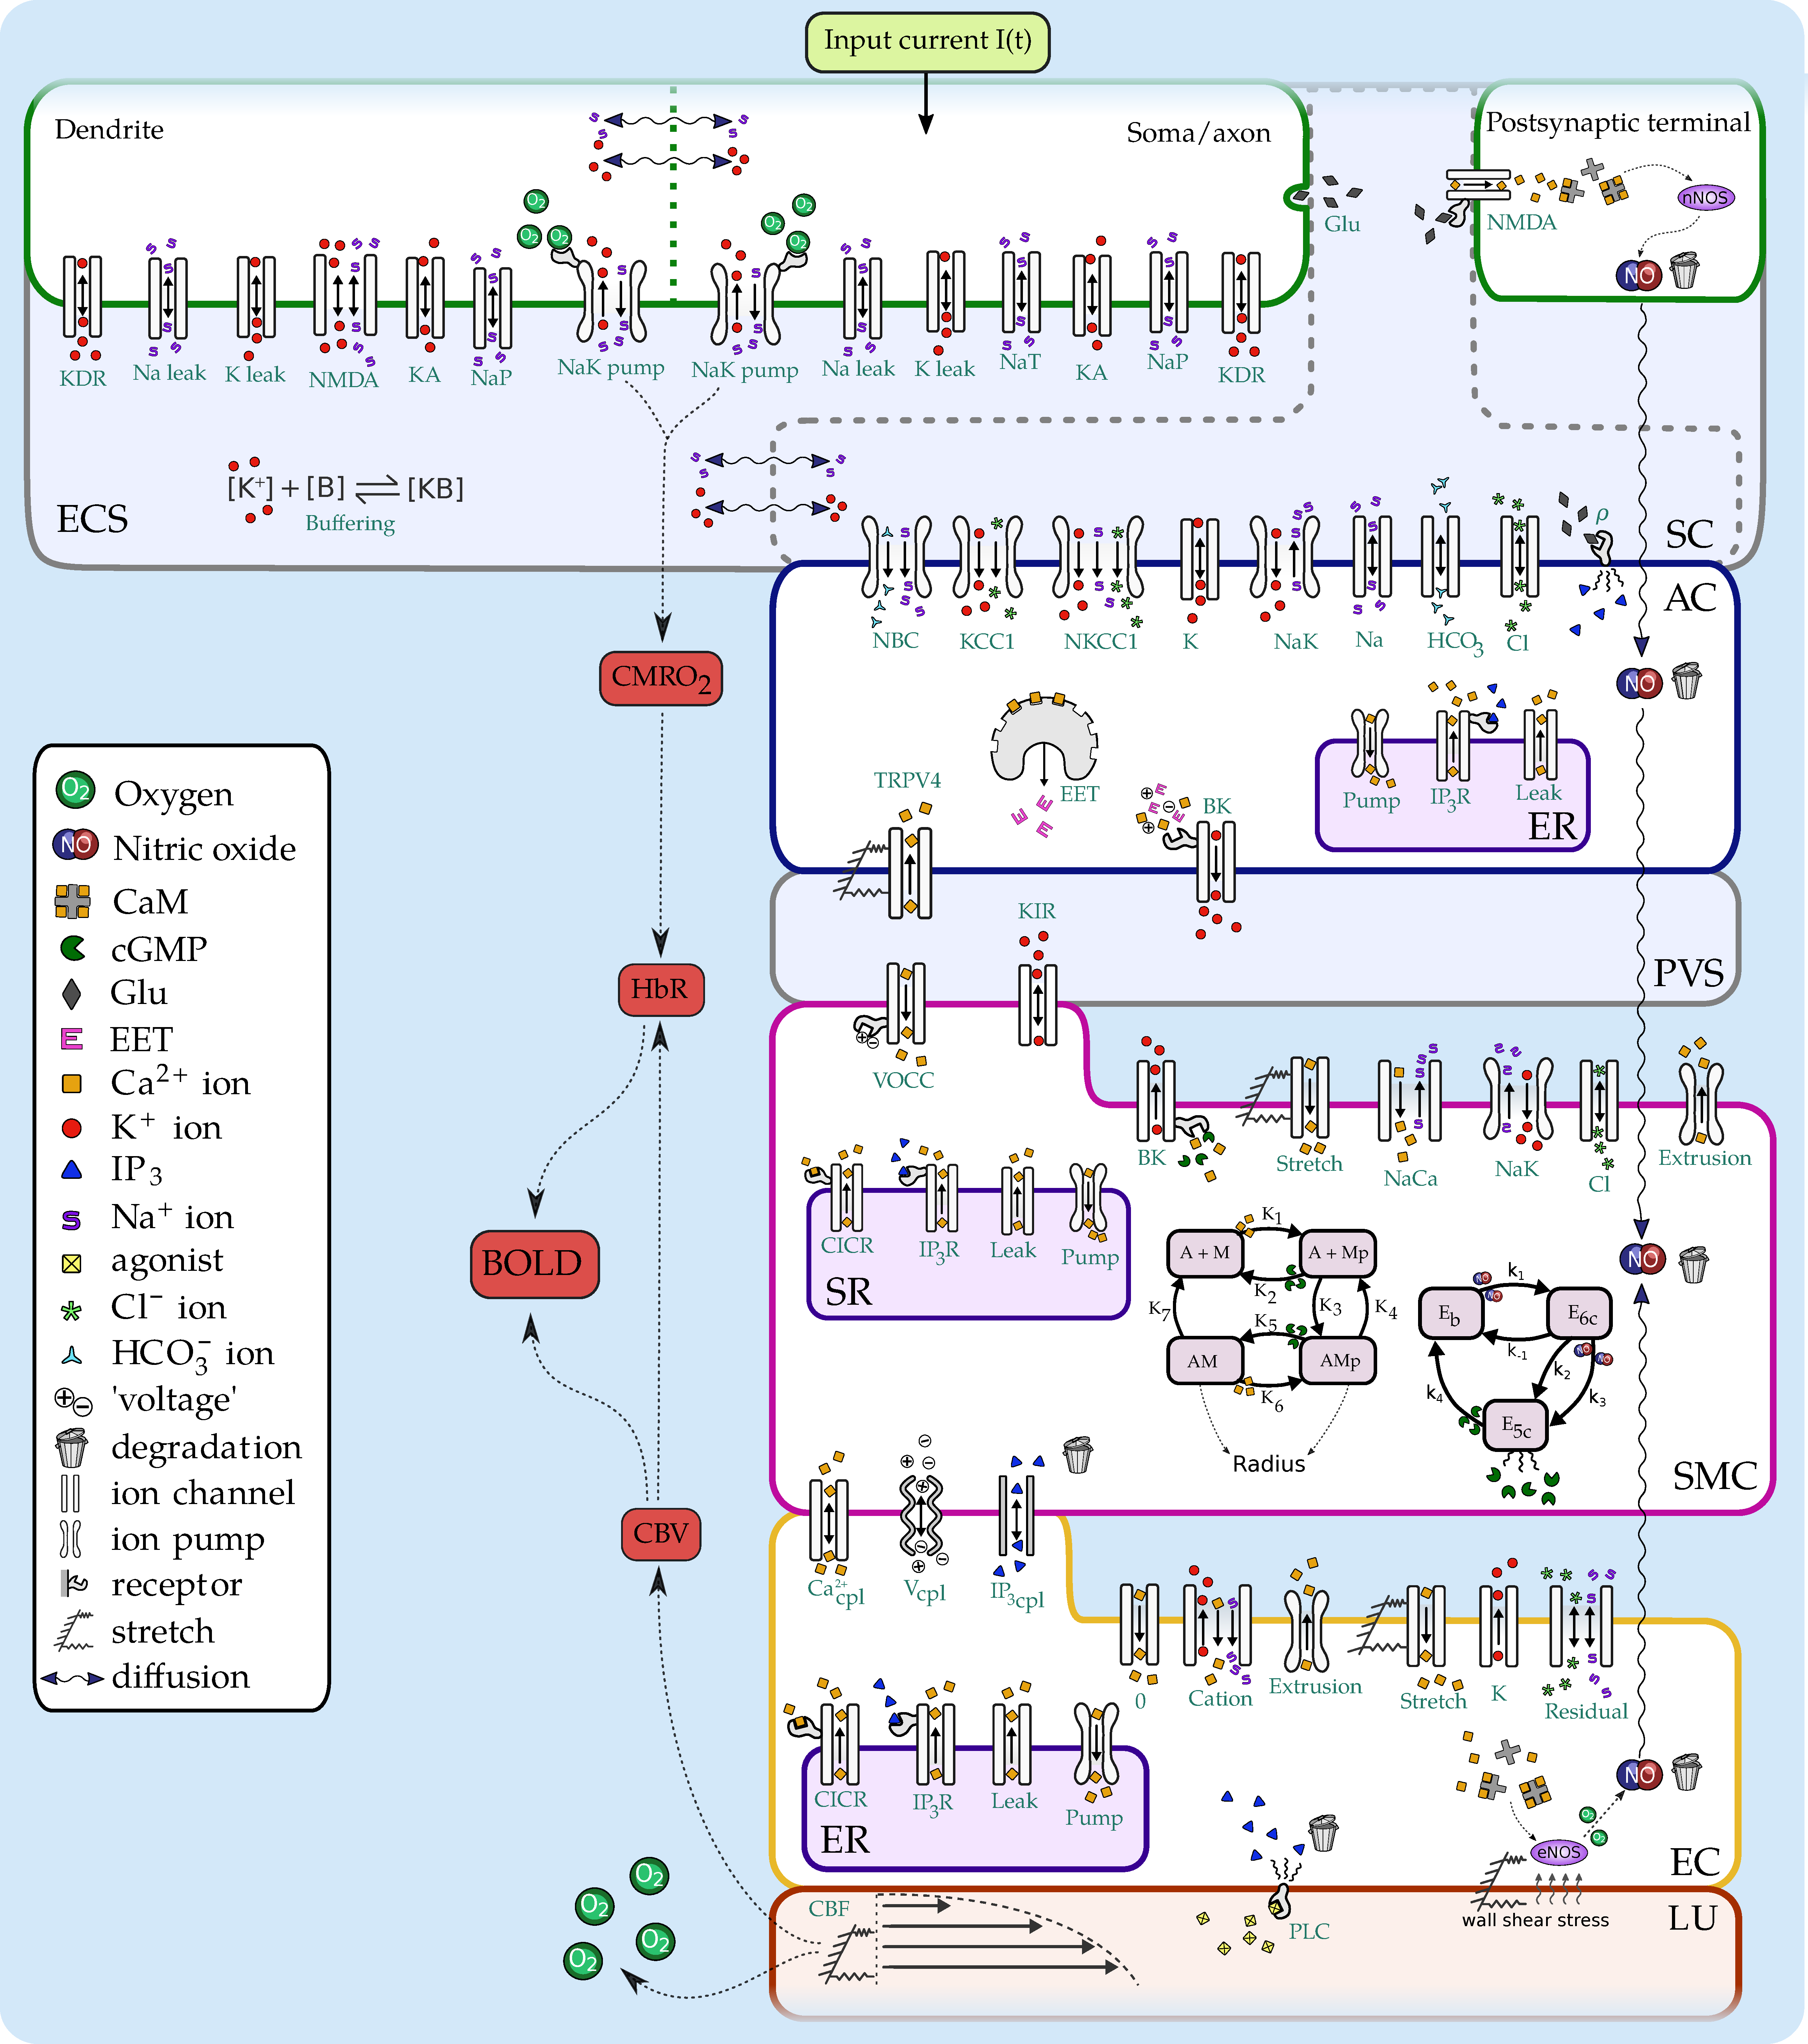
\includegraphics[width=0.8\linewidth]{./nvu_20.pdf}
 				\caption{Schematic of version 1.2}
 				\label{fig:nvu_FULL}
 				\end{figure}

The NO derived from the endothelial cell is mediated by the WSS and the stretch channel providing \Ca which combines with Calmodulin and in a similar manner to nNOS. eNOS is mediated by \Otwo  ~ and L-Arginine to form NO. The NO is then diffused to smooth muscle cell  as is the neuronally derived NO diffused to the astrocyte and thence the SMC.

The full description of the NO pathway is that given in \cite{Dormanns2016b}. 

\textbf{The work of Zheng et al \cite{Zheng2010} showed that as the stimulus period increased the resulting CBF profile showed a concave form. Figure \ref{fig:K+_NO_pathway} is a sketch of the stimulus , the \K in the ECS and the resulting CBF profile. We think that the first part of the concavity is due to the neuron parameters which to some extent provide the driver for the \K in the ECS and synaptic cleft. The second half of the concave profile could be a number of phenomena but we first try to the Nitric Oxide pathway, hence this document.} 
\begin{figure}[h!]
\centering
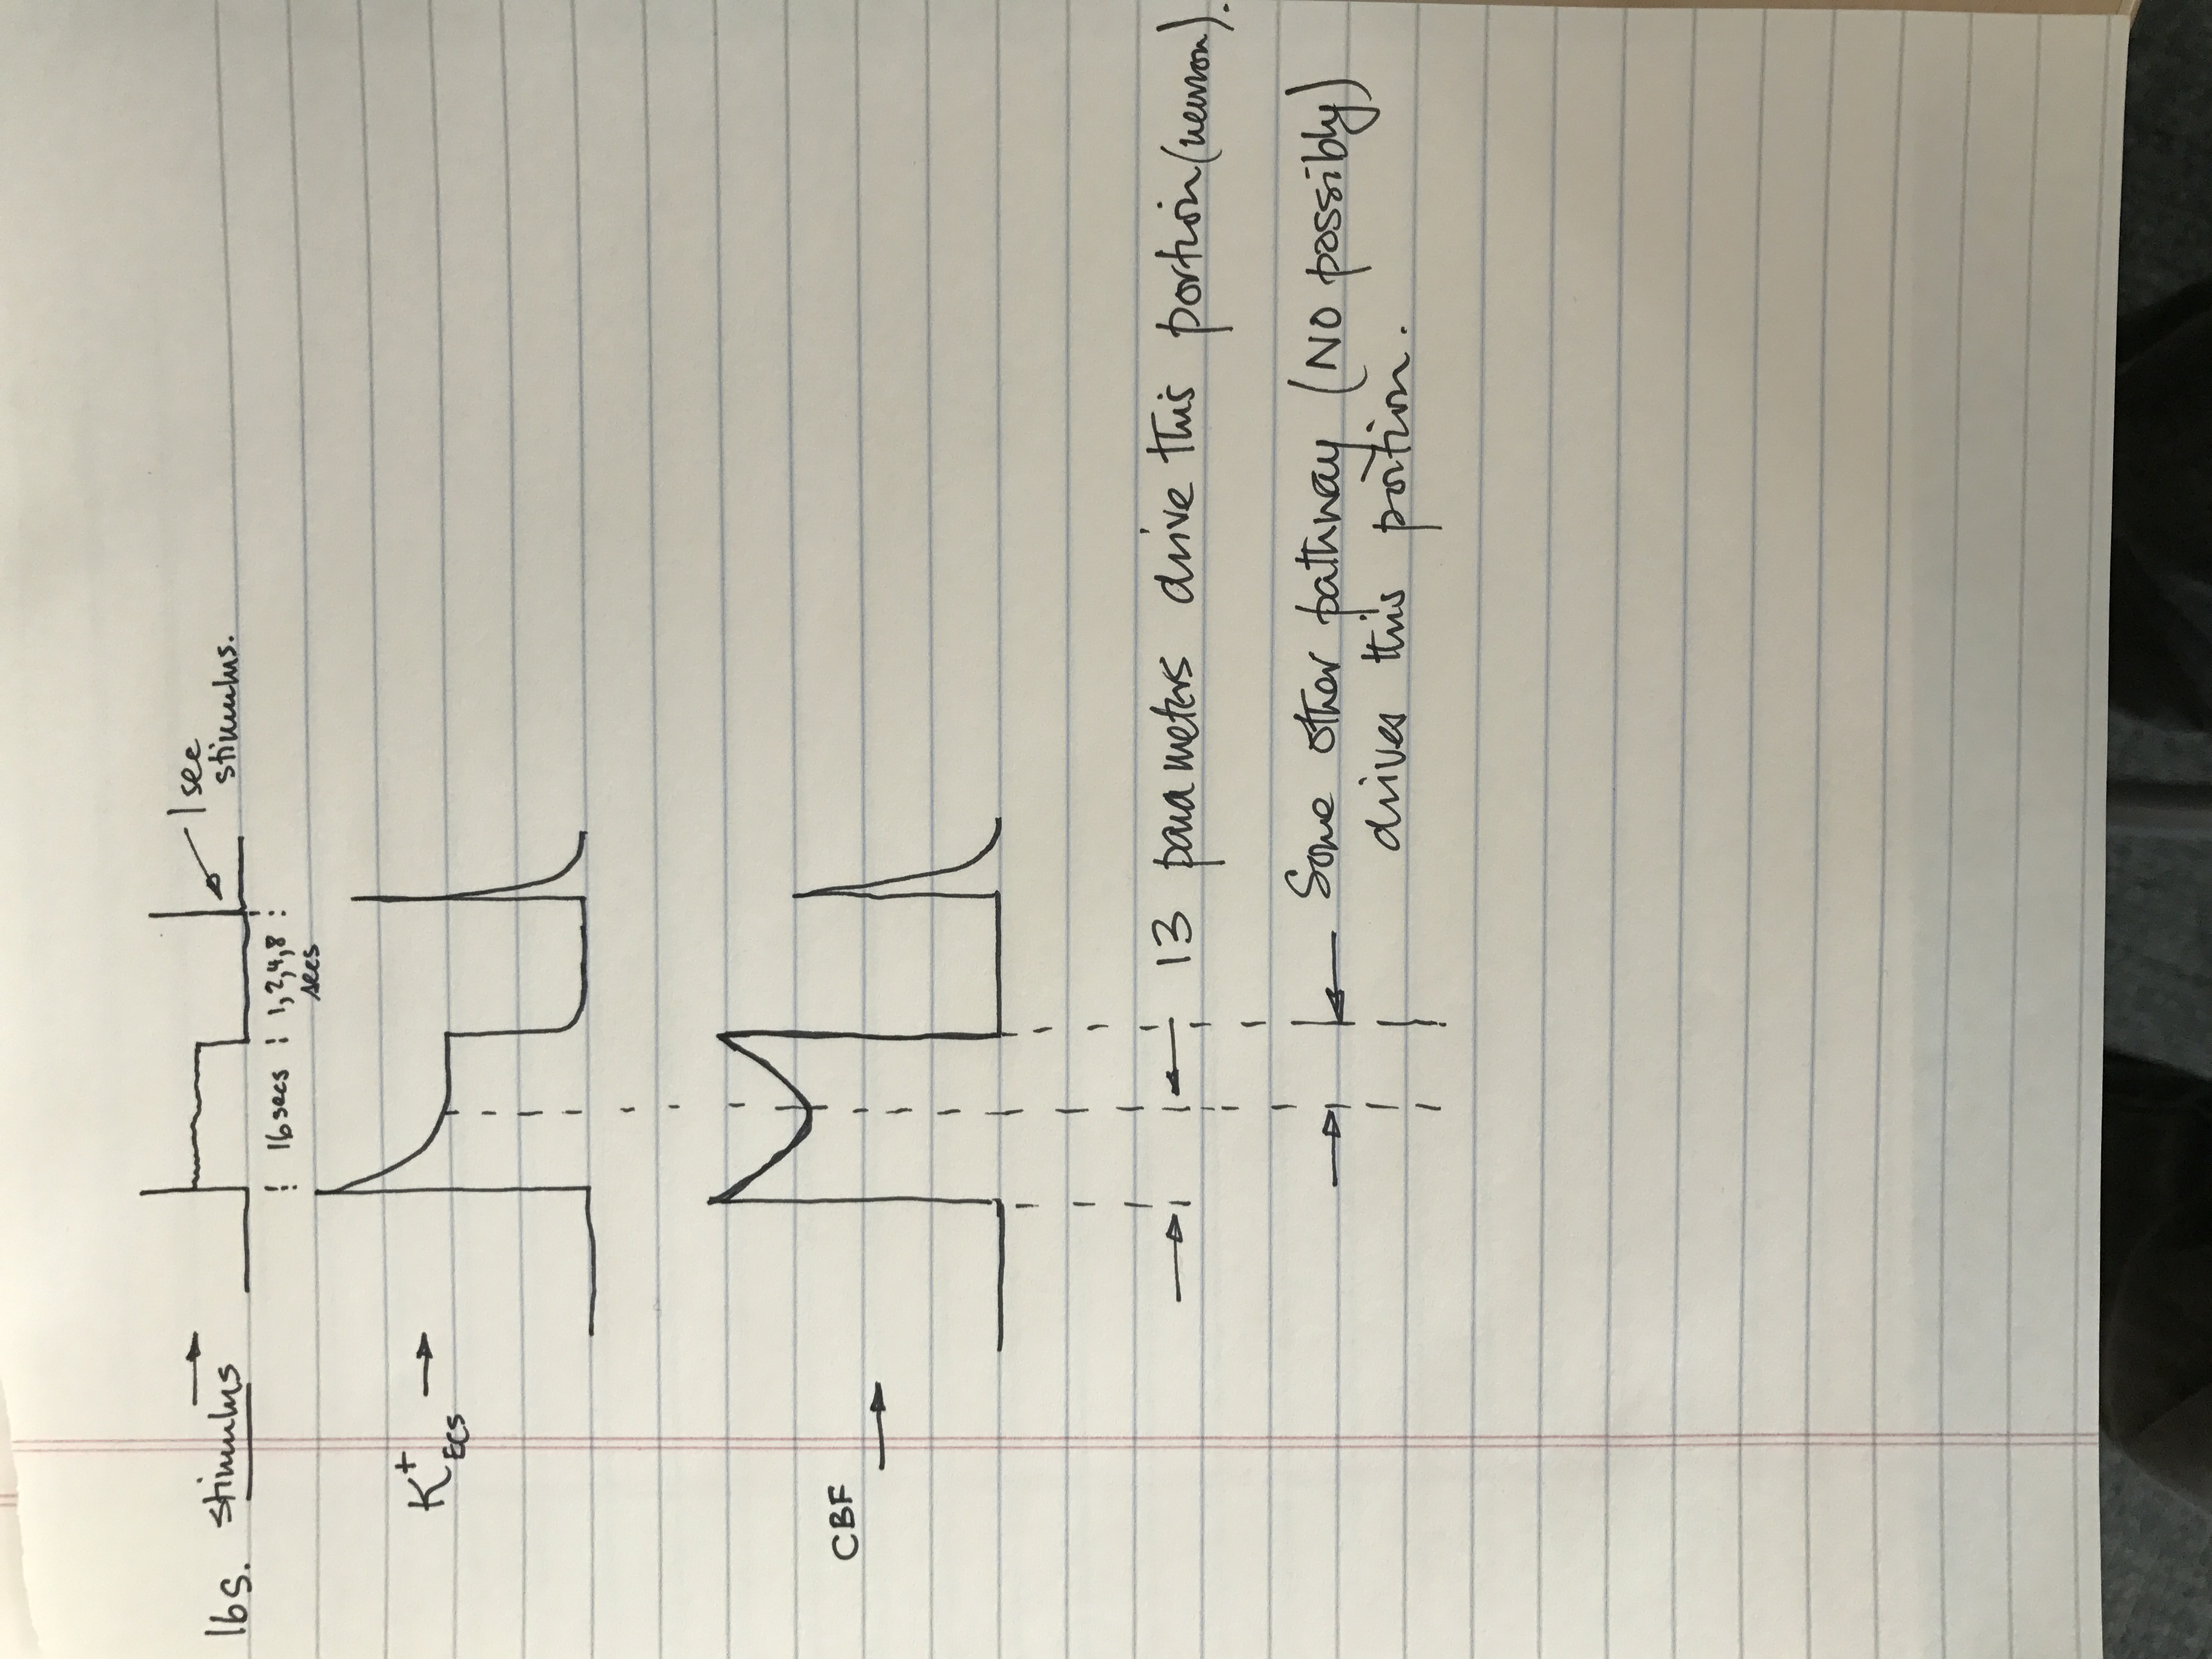
\includegraphics[width=0.7\linewidth, angle =-90]{.//K+_NO_pathway}
\caption{Sketch of 16 second stimulus, \K in the ECS and resulting concave CBF. The second pulse is due to the stimulus profile after the 16 second conditioning block.}
\label{fig:K+_NO_pathway}
\end{figure}

	
\chapter{Basic Equations}
\section{\textbf{Global Constants}}\label{sec:equations}
	\begin{table}[h!]
		\centering
			\begin{tabular}{ p{0.1\linewidth}  >{\footnotesize} p{0.41\linewidth}  >{\footnotesize} p{0.20\linewidth} >{\footnotesize} p{0.27\linewidth} }
			\hline
			$ F $				& Faraday's constant 	& 96500 C mole$^{-1}$ & 	\\
			$ T $				& Temperature				& 300 K				 		&	\\
			$ R_{gas} $	  & Gas constant				& 8.315 J mole K$^{-1}$ &  	\\

			\hline
		\end{tabular}
	\end{table}
				            \section{NO pathway} 
				            \begin{itemize}
				   				 \item           $Ca_n$ :\Ca in the post-synaptic neuron                  
				   				  \item          $nNOS_act_n$ :activated NOS in the post-synaptic neuron
				   				  \item          $NO_n$ : Nitric Oxide in the post-synaptic neuron
				            \end{itemize}

				            
				                        \textbf{ Glutamate input: vesicle released when the extracellular \K is over 5.5 mM ($Ke_{switch}=5.5$) \\}
				            %             Glu = self.shared(t, u);
				                                     %% Glutamate function dependent on neuron membrane potential
				                                     \begin{eqnarray}
				                                     Glu = 0.5 Glu_{switch} \quad Glu_{max}  ( 1 + tanh(  \frac{(K_e - K_{e_{switch}})}{Glu_{slope}}))\\  % based on extracellular K+ (Kager2000) - smooth
				                                     \end{eqnarray}
				                                     \textbf{$Glu_{switch}$ turns the  Glutamate pathway on (=1) or off (=0). }
				                          \begin{eqnarray}
				                         w_{NR2A} &=& \frac{Glu}{(K_{mA} + Glu)}\\%[-] 
				                         w_{NR2B} &=& \frac{Glu}{(K_{mB} + Glu)}\\%[-]           
				                         I_{Ca} &=& -4 v_n  G_M \frac{P_{Ca}}{P_{M}}  \frac{( \frac{Ca_{ex}}{M}))}{(1 + exp(-80 (v_n + 0.02)))} \frac{(exp(2 v_n \frac{F}{RT})))}{(1 - exp(2 v_n \frac{F}{RT})))} \\ %[fA]
				                         I_{Ca_{tot}} &=& I_{Ca} (n_{NR2A}  w_{NR2A} + n_{NR2B}  w_{NR2B})\\ %[fA]
				            %             
				                         CaM &=& \frac{Ca_{n}}{ m_{c}}\\ %[uM]
				                         \tau_{nk} &=&  \frac{x_{nk} ^ 2}{2  D_{cNO}}\\ %[s]
				            %             
				            \end{eqnarray}
				            \textbf{NO production flux (\uMpers):}
				            \begin{eqnarray}
				                        p_{NO_{n}} &=& NO_{switch}   nNOS_{act_{n}} V_{max_{NO_{n}}}  \frac{O2_{n}}{K_{mO2_{n}} + O2_n}  \frac{LArg_{n}}{K_{mArg_{n}} + LArg_{n}}\\ %[uM/s]
				            \end{eqnarray}
			\textbf{	NO consumption flux (\uMpers):}
				\begin{eqnarray}
				                         c_{NO_{n}} &=& k_{O2_{n}}  (NO_{n})^2 O2_{n}\\ %[uM/s]
				\end{eqnarray}
\textbf{				NO diffusive flux (\uMpers):}
				\begin{eqnarray}
				                         d_{NO_{n}} &=& \frac{NO_{k} - NO_{n}}{\tau_{nk}}\\ %[uM/s]
				\end{eqnarray}

				                          
				            \textbf{$NO_{switch}$ turns the NO Pathway on or off}
				            
\chapter{Conservation equations}
\section{post-synaptic neuron}
\begin{eqnarray}
\frac{d [Ca]_{n}}{dt}&=&  \frac{( \frac{I_{Ca_{tot}}}{2 F V_{spine}}  - (k_{ex}  (Ca_{n} - Ca_{rest})))}{1 + \lambda_{buf}}\\%[uM/s]
 \frac{d  [nNOS_{act}]_{n}}{dt} &=&  \frac{V_{maxNOS}  CaM }{K_{actNOS} + CaM} -\mu _{2_{n}}  nNOS_{{act}_{n}}\\ %[uM/s]
%            du(idx.NO_n, :) &=& p_NO_n - c_NO_n + d_NO_n; %[uM/s]
\end{eqnarray}

\section{Astrocyte}
	\textbf{Rate of change of astrocytic NO concentration }(\uMpers):
	       		\begin{equation}  
	      			 \dfrac{\mathrm{d}\NOk}{\mathrm{d}t} = \pNO{k} - \cNO{k} + \dNO{k}
				\end{equation}   
	
			\subsubsection*{Algebraic equations}
				NO production flux (\uMpers):
				\begin{equation} 
					\pNO{k} = 0
				\end{equation}
			
				NO consumption flux (\uMpers):
				\begin{equation} 
					\cNO{k} = k_{\text{O2},k} [\NO]_k^2 [\Otwo]_k
				\end{equation}
					
				NO diffusive flux (\uMpers):
				\begin{equation} 
					\dNO{k} = \frac{[\NO]_n - [\NO]_k}{\tau_{nk}} + \frac{[\NO]_i - [\NO]_k}{\tau_{ki}}
				\end{equation}	
					
				Time for NO to diffuse between the centres of the AC and the SMC (s):
				\begin{equation}
					\tau_{ki} = \frac{x_{ki}^2}{2 D_{\text{c,NO}}}
				\end{equation}
				
	%		\subsubsection*{Constants}
				\begin{table}[h!]
					\centering
					\begin{tabular}{ p{0.07\linewidth}  >{\footnotesize} p{0.47\linewidth}  >{\footnotesize} p{0.17\linewidth} >{\footnotesize} p{0.17\linewidth} }
						\hline
						$ k_{\text{O2},k} $ 	& \Otwo\ reaction rate constant							& 9.6\e{-6}\uM$^{-2}$s\n 	& \citep{Kavdia2002} \\ % converted from 9.6e6 M^-2 s^-1
						$ x_{ki} $ 				& distance between centres of AC and SMC compartments 	& 25 \textmu m 				& model assumption \\ 
						$[\Otwo]_k$    & oxygen concentration in the astrocyte & 200 \uM 			& M.E. \\
						\hline
					\end{tabular}
				\end{table}
				
				
\section{Smooth Muscle cell}
%Calcium flux through the stretch-activated channels in the SMC (in \uMs): 
%	\begin{equation} \label{eq:Jstretchi}
%	\begin{split}
%	J_{stretch_{i}}= \frac{G_{stretch}}{1+ exp\left(-\alpha_{stretch}  \left(  \frac{\Delta pR}{h} -\sigma_{0}   \right) \right)}  \left(  v_{i}-E_{SAC}   \right) 
%	\end{split}
%	\end{equation}
%	%
%	\begin{table}[h!]
%	\centering
%	\begin{tabular}{ p{0.09\linewidth}  >{\footnotesize} p{0.5\linewidth}  >{\footnotesize} p{0.27\linewidth} >{\footnotesize} p{0.03\linewidth} }
%	\hline
%	$G_{stretch}$      		& Whole cell conductance for SACs						& 6.1$\times$10$^{-3}$ \uMpmVs	&\cite{Koenigsberger2006} \\
%	$\alpha_{stretch}$      & Slope of stress dependence of the SAC activation sigmoidal	& 7.4$\times$10$^{-3}$ \pmmHg	&\cite{Koenigsberger2006} \\
%	$ \Delta p $			& Pressure difference										& 30 \mmHg			& ME \\
%	$\sigma_{0}$      		& Half-point of the SAC activation sigmoidal				& 500 \mmHg			&\cite{Koenigsberger2006} \\
%	$E_{SAC}$      			& Reversal potential for SACs							& -18 \mV			&\cite{Koenigsberger2006} \\
%	\hline
%	\end{tabular}
%	\label{tab:Jstretchi}
%	\end{table}
		Rate of change of NO concentration in the SMC (\uMpers):
				    \begin{equation}  
		      			 \dfrac{\mathrm{d}\NOi}{\mathrm{d}t} = \pNO{i} - \cNO{i} + \dNO{i} 
					\end{equation}
					
					Rate of change of fraction of sGC in the basal state (s\n):% Yang2005
					\begin{equation} 
						\dfrac{\mathrm{d}E_b}{\mathrm{d}t} = -k_1 E_b [\NO]_i + k_{-1} E_{6c} + k_4 E_{5c}
					\end{equation}	
					
					Rate of change of fraction of sGC in the intermediate form (s\n):% Yang2005
					\begin{equation} 
		%				\dfrac{\mathrm{d}E_{6c}}{\mathrm{d}t} = k_1 E_b [\NO]_i - k_{-1} E_{6c} - k_2 E_{6c} - k_3 E_{6c} [\NO]_i
						\dfrac{\mathrm{d}E_{6c}}{\mathrm{d}t} = k_1 E_b [\NO]_i - (k_{-1} + k_2) E_{6c} - k_3 E_{6c} [\NO]_i
					\end{equation}	
		
					Rate of change of cGMP concentration (\uMpers):		% Yang2005	
					\begin{equation} 
						\dfrac{\mathrm{d}[\cGMP]_i}{\mathrm{d}t} = V_{\text{max,sGC}} E_{5c} - \frac{V_{\text{max,pde}}[\cGMP]_i}{K_{\text{m,pde}}+[\cGMP]_i}
					\end{equation}	
					
					
						Maximum cGMP production rate (\uMpers):
									\begin{equation}
										V_{\text{max,pde}} = k_{\text{pde}} [\text{cGMP}]_i
									\end{equation}
		       		
				\subsubsection*{Algebraic equations}
					NO production flux (\uMpers):
					\begin{equation} 
						\pNO{i} = 0
					\end{equation}
				
					NO consumption flux (\uMpers):
					\begin{equation} 
						\cNO{i} = k_{\text{dno}} [\NO]_i
					\end{equation}
		
					NO diffusive flux (\uMpers):
					\begin{equation} 
						\dNO{i} = \frac{[\NO]_k - [\NO]_i}{\tau_{ki}} + \frac{[\NO]_j - [\NO]_i}{\tau_{ij}}
					\end{equation}
		
						\begin{eqnarray} 
							\tau_{i,j}=\frac{x_{K,i}^2}{2 D_{NO}}\\
							x_{K,i}=25 \mu m \\
						\end{eqnarray}
					sGC kinetics rate constant (s\n): % Yang2005
					\begin{equation} 
						k_4 = C_4 [\cGMP]_i^{m_{4}}
					\end{equation}	
					
					Fraction of sGC in the fully activated form (dim.less):% Yang2005
					\begin{equation} 
						E_{5c} = 1 - E_b - E_{6c}
					\end{equation}	
					
					Regulatory effect of cGMP on myosin dephosphorylation (dim.less):			%not on the BK channel open probability !
					\begin{equation} 
						R_{\text{cGMP}} = \frac{[\text{cGMP}]_i^2}{K_{\text{m,mlcp}}^2 + [\text{cGMP}]_i^2}
					\end{equation}
					
					Rate constants for dephosphorylation (s\n ) in the Hia and Murphy 4-state latch model, see \citet{Dormanns2016b}:
					\begin{equation} 
						K_{2c} = K_{5c} = \delta_i \left(k_{\text{mlpc,b}} + k_{\text{mlpc,c}} R_{\text{cGMP}}\right)
					\end{equation}	
			
				Equilibrium distribution of open channel states for the BK channel flux into the ECS  (dim.less), see \citet{Dormanns2014}:  % Koenigsberger
							\begin{equation} 
								K_{\text{act},i} = \frac{(\Cai + c_{\text{w},i})^2}{(\Cai + c_{\text{w},i})^2 + \beta_i \exp(v_{\text{Ca}3,i} - v_i/R_{\text{K},i} )}
							\end{equation}
							
							Translation factor, regulatory effect of cGMP on the BK channel open probability (\uM)):			
			%				\begin{equation} 
			%					c_{\text{w},i} = \frac{1}{\epsilon_i + \alpha_i \exp(\gamma_i [\text{cGMP}]_i)}
			%				\end{equation}
							\begin{equation} 
								c_{\text{w},i} = \frac{c_{w,max}}{2}[1 + tanh( \frac{[\text{cGMP}_i]-\epsilon_i}{\alpha_i})]
							\end{equation}
							
							Time for NO to diffuse between the centres of the SMC and the EC (s):
							\begin{equation}
								\tau_{ij} = \frac{x_{ij}^2}{2 D_{\text{c,NO}}}
							\end{equation}

									

\section{Endothelial Cell}
	\begin{equation} 
	%				\dfrac{\mathrm{d}[\eNOSact]_j}{\mathrm{d}t} = \gamma_{\text{eNOS}} A_{\text{eNOS,Ca}} + (1-\gamma_{\text{eNOS}}) A_{\text{eNOS,wss}} - \mu_{\text{deact},j}[\eNOSact]_j
					\dfrac{\mathrm{d}[\eNOSact]_j}{\mathrm{d}t} = \gamma_{\text{eNOS}} \frac{K_{\text{dis}}[\Ca]_j}{K_{\text{m,eNOS}}+[\Ca]_j} + (1-\gamma_{\text{eNOS}}) g_{\max} F_{\text{wss}}   - \mu_{\text{deact},j}[\eNOSact]_j
				\end{equation}	
						
				\begin{equation} 
					\dfrac{\mathrm{d}\NOj}{\mathrm{d}t} = \pNO{j} - \cNO{j} + \dNO{j} 
				\end{equation}
				NO production flux (\uMpers):
				\begin{equation} 
					\pNO{j} = V_{\text{max,NO},j} [\eNOSact]_j  \frac{[\Otwo]_j}{K_{\text{m,O2},j}+[\Otwo]_j} \frac{[\LArg]_j}{K_{\text{m,L-Arg},j}+[\LArg]_j}
				\end{equation}	
				
				NO consumption flux (\uMpers):
				\begin{equation} 
					\cNO{j} = k_{\text{O2},j} [\NO]_j^2 [\Otwo]_j 
				\end{equation}	
				
				NO diffusive flux (\uMpers):					
				\begin{equation} 
					\dNO{j} = \frac{[\NO]_i - [\NO]_j}{\tau_{ij}} - \frac{4 D_{\text{c,NO}}[\NO]_j}{r^2}
				\end{equation}	

							\begin{eqnarray}
							\tau_{ij}=\frac{x^2}{2D_{NO}}\\
							x=3.75 \mu m
							\end{eqnarray}

	\subsubsection*{Algebraic equations}
	
	%			\Ca -dependent eNOS activation flux (\uMpers):
	%			\begin{equation}
	%				A_{\text{eNOS,Ca}} = \frac{K_{\text{dis}}[\Ca]_j}{K_{\text{m,eNOS}}+[\Ca]_j}
	%			\end{equation}
				
	%			Wall-shear-stress-dependent eNOS activation flux (\uMpers):
	%			\begin{equation}
	%				A_{\text{eNOS,wss}} = g_{\max} F_{\text{wss}}      
	%			\end{equation}
				
				Fraction of the elastic strain energy stored within the membrane (dim.less): % Comerford2008 / Wiesner1997 unit??
				\begin{equation} 
					F_{\text{wss}} = \frac{1}{1+\alpha_{\text{wss}} \exp(-W_{\text{wss}})} - \frac{1}{1+\alpha_{\text{wss}}}
				\end{equation}	
				
				Strain energy density (Pa): % Comerford2008 / Wiesner1997	unit??	
				\begin{equation} 
					W_{\text{wss}} = W_0 \frac{(\tau_{\text{wss}} + \sqrt{16 \delta_{\text{wss}}^2 + \tau_{\text{wss}}^2} - 4 \delta_{\text{wss}})^2}{\tau_{\text{wss}} + \sqrt{16\delta_{\text{wss}}^2 + \tau_{\text{wss}}^2}}
				\end{equation}	
				
				Wall shear stress (Pa): % unit??
				\begin{equation}
	%				\tau_{\text{wss}} = \frac{4 \eta Q}{\pi r^3} = \frac{r \Delta P}{2 L}
					\tau_{\text{wss}} = \frac{r \Delta P}{2 L}
				\end{equation}
				
	%			Blood flow (unit??):
	%			\begin{equation}
	%				Q = \frac{\Delta P \pi r^4}{8 \eta L}
	%			\end{equation}	
					
	%dy(ind.NO_j)  =  (V_NOj_max * (state(ind.eNOS_act)) * (Oj/(K_mO2_j+Oj)) * (LArg_j/(K_mArg+LArg_j)) ) + 
	%((state(ind.NO_i)-state(ind.NO_j))/tau_ij)   - k_O2*(state(ind.NO_j))^2*Oj - state(ind.NO_j)*4*3300/(25^2);
	
	
\chapter{parameter listing}
				%		\subsubsection*{Constants}
							\begin{table}[h!] \label{tab:sGC}
								\centering
								\begin{tabular}{ p{0.1\linewidth}  >{\footnotesize} p{0.41\linewidth}  >{\footnotesize} p{0.14\linewidth} >{\footnotesize} p{0.26\linewidth} }
									\hline
									$ k_{-1} $ 				& sGC kinetics rate constant 	& 100 s\n 				& \citep{Yang2005} \\ 
									$ k_1 $ 				& sGC kinetics rate constant 	& 2\e{3} \uM\n\ s\n 		& \citep{Yang2005} \\ 
									$ k_2 $ 				& sGC kinetics rate constant 	& 0.1 s\n 				& \citep{Yang2005} \\ 
									$ k_3 $ 				& sGC kinetics rate constant 	& 3 \uM\n\ s\n 			& \citep{Yang2005} \\ 
									$ V_{\text{max,sGC}} $ 	& maximal cGMP production rate	& 0.8520 \uMpers  		& \citep{Yang2005} \\ 
									$ K_{\text{m,pde}} $ 	& Michaelis constant 			& 2 \uM 				& \citep{Yang2005} \\ 
									$ k_{\text{dno}}$ 		& lumped NO consumption rate constant reflecting the activity of various NO scavengers & 0.01 s\n & \citep{Yang2005} \\ 
									$ C_4 $ 				& constant 						& 0.011 s\n\ \uM$^{-2}$ 	& \citep{Yang2005} \\ 
									$ m_4 $ 				& cGMP feedback strength 		& 2 (dim.less) 			& \citep{Yang2005} \\
									$ K_{\text{m,mlcp}} $ 	& Hill coefficient				& 5.5 \uM 				& \citep{Yang2005} \\
									$ \delta_i $ 			& constant to fit data			& 58.1395 (dim.less)	& \citep{Hai1988}, fit\\
									$ k_{\text{mlpc,b}} $ 	& basal MLC dephosphorylation rate constant			& 0.0086 s\n  			& \citep{Yang2005} \\
									$ k_{\text{mlpc,c}} $ 	& first-order rate constant for \cGMP-regulated MLC dephosphorylation		& 0.0327 s\n 			& \citep{Yang2005} \\
									$ \alpha_i $ 			& constant to fit data			& 0.665 \uM  		&  \citep{Stockand1996}\\  % shoul be dimless??
									$ \beta_i $ 			& translation factor for membrane potential dependence of $ K_{\text{Ca}} $ channel activation sigmoidal & 0.13 \uM$^2$ & \citep{Koenigsberger2006} \\ 
									$ c_{w,max} $ 			& constant to fit data & 1 \uMpers & \citep{Stockand1996}\\ 
									$ \epsilon_i$			& constant to fit data 				& 10.75 \uM 	&  \citep{Stockand1996} \\ 
									$ \Cai $ 				& calcium concentration in the SMC cytosol & var. 		& see \citet{Dormanns2014} \\
									$ v_{\text{Ca}3,i} $ 			& half-point for the $ K_{\text{Ca}} $ channel activation sigmoidal. & -27 mV & \citep{Koenigsberger2006}\\ 
									$ v_i $ 				& SMC membrane potential 		& var. 	& see \citep{Dormanns2014} \\
									$ R_{\text{K},i}  $ 				& Maximum slope of the $K_{Ca}$ activation sigmoidal & 12 mV & \citep{Koenigsberger2006}\\ 
									$ k_{\text{pde}} $		& phosphodiesterase rate constant & 0.0195 s\n & \citep{Yang2005} \\
									\hline
								\end{tabular}
							\end{table}	
											%					$ \gamma_{eNOS} $ 	&  &  \\ 
											%					$ [\Otwo]_j $ 		&  &  \\ 
											%					$ [\LArg]_j $ 		&  &  \\ 
											%					$V_{NO,j_{max}}$			& Maximum eNOS catalytic rate	& \unit[0.24]{\uMpers}	&  M.E.\footnotemark on basis of \citep{Chen2006a}  \\
											%					$K_{m,j}^{O_2}$ 			& Michaelis constant for \Otwo 				& \unit[0.24]{\uMpers}	&    \\
											%					$K_{m,j}^{L\text{-}Arg}$ 	& Start of back-buffering				& \unit[0.24]{\uMpers}	&    \\
     NO pathway in Neuron 
\begin{itemize}
    \item Parameter  ('$m_c$', 4);     \textbf{DON'T CHANGE THIS !!!} [-] Number of Ca2+ bound per calmodulin (approximated as parameter, originally an algebraic variable that changed from 3.999 to 4)\\
    \item Parameter  ('$K_{mA}$', 650);           [uM] - fit to Santucci2008\\
    \item Parameter ('$K_{mB}$', 2800);          [uM] - fit to Santucci2008\\
    \item Parameter  ('$v_n$', -0.04);           [V] ; \textbf{DON'T CHANGE THIS !!!}the neuronal membrane potential , assumed to be approx constant in this model\\
    \item Parameter  ('$G_M$', 46000);          [fS]! was 46 pS! ; the conductance of the NMDA channel to Ca2+ compared  \\
    \item Parameter  ('$P_{Ca_{P_{M}}}$', 3.6);        [-] ; the relative conductance of the NMDA channel to Ca2+ compared to monovalent ions\\
    \item Parameter  ('$Ca_{ex}$', 2e3);           [microM] ; the external calcium concentration (in Comerford+David2008: 1.5 mM!)\\
    \item Parameter  ('M', 1.3e5);             [microM] ; the concentration of monovalent ions in the neuron\\
    \item Parameter  ('$n_{NR2A}$', 0.63);         [-] ; average number of NR2A NMDA receptors per synapse (Santucci2008)\\
    \item Parameter  ('$n_{NR2B}$', 11);          [-] ; average number of NR2B NMDA receptors per synapse (Santucci2008)\\
    \item Parameter  ('$V_{max_{NO_{n}}}$', 4.22);     [$s^-1$] ; maximum catalytic rate of NO production (Chen2006) - obtained from fig 6 and equ 17 and 18\\
    \item Parameter  ('$O2_n$', 200);            [uM] ; tissue O2 concentration in the neuron (M.E.)\\
    \item Parameter  ('$K_{mO2_{n}}$', 243);         [uM] ; Chen2006\\
    \item Parameter  ('$LArg_n$', 100);          [uM] ; \\
    \item Parameter  ('$K_{mArg_{n}}$', 1.5);        [uM] ; \\
    \item Parameter  ('$k_{O2_{n}}$', 9.6e-6);       [$uM^-2 s^-1$] ; % (Kavdia2002)
    \item Parameter  ('$x_{nk}'$, 25);             [um] ;  (M.E.)
    \item Parameter  ('$D_{cNO}$', 3300);          [$um^2 s^-1$] ; Diffusion coefficient NO (Malinski1993)
    \item Parameter  ('$V_{spine}$', 8e-8);        [nL] ; volume of the neuronal dendritic spine Santucci2008\\
    \item Parameter  ('$k_{ex}$', 1600);           [$s^-1$] ; decay rate constant of internal calcium concentration Santucci2008\\
    \item Parameter  ('$Ca_{rest}$', 0.1);         [$uM$] ; resting calcium concentration (in Comerford and David2008: 2.830 mM; in Santucci2008P: 0.1 $\mu M$)\\
    \item Parameter  ('$lambda_{buf}$', 20);       [-] ; buffer capacity Santucci2008\\
    \item Parameter  ('$V_{maxNOS}$', 25e-3);      [] ; M.E.\\
    \item Parameter  ('$K_{actNOS}$', 9.27e-2);    [uM] ; \\
    \item Parameter  ('$mu2_n$', 0.0167);        [$s^-1$] ; rate constant at which the nNOS is deactivated Comerford2008\\
\end{itemize}

\textbf{NO pathway parameters in Astrocyte}

\begin{itemize}
    \item  Parameter  ('$D_{cNO}$', 3300);          [$um^2 s^-1$] ; Diffusion coefficient NO (Malinski1993)\\
    \item  Parameter  ('$x_{nk}$', 25);             [um] ;  (M.E.)\\
    \item  Parameter  ('$x_{ki}$', 25);             [um] ;  (M.E.)\\
    \item Parameter  ('$k_{O2_{k}}$', 9.6e-6);       [$uM^-2 s^-1$] ;  (Kavdia2002)\\
    \item  Parameter  ('$O2_k$', 200);            [uM] ;  (M.E.)
\end{itemize}

\textbf{NO pathway parameters in Smooth Muscle Cell and Endothelial Cell}
\begin{itemize}
    \item  Parameter   ('$D_{cNO}$', 3300);  [$um^2 s^-1$] ; Diffusion coefficient NO (Malinski1993)\\
    \item  Parameter   ('$K_{mArg_{j}}$', 1.5);  [] ;\\
    \item  Parameter   ('$K_{mO2_{j}}$', 7.7);  [] ; Chen2006\\
    \item  Parameter   ('$k_{dno}$', 0.01);  [$s^{-1}$] ;\\
    \item  Parameter   ('$K_{m_{mlcp}}$', 5.5);  [uM] ;\\
    \item  Parameter   ('$V_{NOj_{max}}$', 1.22);  [$s^{-1}$] ; maximum catalytic rate of NO production (Chen2006) - obtained from fig 6 and equ 17 and 18\\
    \item  Parameter   ('$O2_j$', 200);  [uM] ; O2 concentration in the EC (ME)\\
    \item  Parameter   ('$LArg_j$', 100);  [uM] ;\\
    \item  Parameter   ('$k_{O2}$', 9.6e-6);  [$uM^-2 s^{-1}$] ;\\
    \item  Parameter   ('$W_0$', 1.4);  [$Pa^{-1}$] ; shear gating constant (Comerford2008)\\
    \item  Parameter   ('$delta_{wss}$', 2.86);  [Pa] ; the membrane shear modulus (Comerford2008)\\
    \item  Parameter   ('$k_1$', 100);  [$s^{-1}$] ;\\
    \item  Parameter   ('k1', 2e3); [$uM^{-1} s^{-1}$] ;\\
    \item  Parameter   ('k2', 0.1);  [$s^{-1}$] ;\\
    \item  Parameter   ('k3', 3);  [$uM^{-1} s^{-1}$] ;\\
    \item  Parameter   ('$V_{max_{sGC}}$', 0.8520);  [] ;\\
    \item  Parameter   ('$k_{pde}$', 0.0195);  [$s^{-1}$] ;\\
    \item  Parameter   ('$C_4$', 0.011);  [$s^{-1} microM^{-2}$] ;\\
    \item  Parameter   ('$K_{m_{pde}}$, 2);  [uM] ;\\
    \item  Parameter   ('$gam_{eNOS}$', 0.1);  [-] ;\\
    \item  Parameter   ('$mu2_j$', 0.0167);  [$s^{-1}$] ;\\
    \item  Parameter   ('$K_{dis}$', 9e-2);  [$uM s^{-1}$] ;\\
    \item  Parameter   ('$K_{eNOS}$', 4.5e-1);  [uM] ;    \\
    \item Parameter   ('$g_{max}$', 0.06);  [uM $s^{-1}$] ;    \\
    \item  Parameter   ('alp', 2);  [-] ; zero shear open channel constant (Comerford2008); in Wiesner1997: alp = 3\\
    \item  Parameter   ('$delta_{p_{L}}$', 9.1e4);  9.1e4: ME\\
    \item  Parameter   ('$x_{ki}$', 25);  [um]  (M.E.)\\
    \item  Parameter   ('$x_{ij}$', 3.75);  [um]  (Kavdia2002)\\
\end{itemize}
\bibliography{JTB_library,mybibfile,/Users/timdavid/Documents/MendeleyDesktop/library,library_part_I}

\end{document}